\documentclass{article}
\usepackage{amsmath}
\usepackage{xcolor}
\usepackage[margin=1in]{geometry}
\usepackage{graphicx}
\usepackage{mdframed}
\usepackage{float}
\usepackage{xcolor}
\usepackage{tikz}

\definecolor{solutionblue}{RGB}{0,0,255}
\usetikzlibrary{plotmarks}

\begin{document}

% Header
\begin{center}
    \textbf{\LARGE Assignment 8} \\[1ex]
    \textbf{ECE 360} \\[1ex]
    \textbf{V00984826} \\[2ex]
\end{center}

% Question and Solution Template

% Example Question and Solution (B-7-1, S-7-1)
\section*{B-7-X}
\section*{S-7-X}
\section*{B-7-X}
\section*{S-7-X}
\section*{B-7-X}
\section*{S-7-X}
\section*{B-7-X}
\section*{S-7-X}
\end{document}

% Question text
% EXAMPLE TEXT
% Insert question image if needed
%\begin{center}
%    \includegraphics[width=0.8\textwidth]{image_B-7-1} % Replace "image_B-7-1" with the actual filename
%\end{center}
%The following MATLAB program produces the Bode diagram shown below.
%
%\begin{mdframed}
%{\color{solutionblue}
%\begin{verbatim}
%% ***** Bode diagram *****
%num = [0 10 4 10];
%den = [1 0.8 9 0];
%bode(num, den)
%title('Bode Diagram of G(s) = 10(s^2 + 0.4s + 1)/[s(s^2 + 0.8s + 9)]')
%\end{verbatim}}
%\end{mdframed}
%\begin{figure}[H]
%    \centering
%    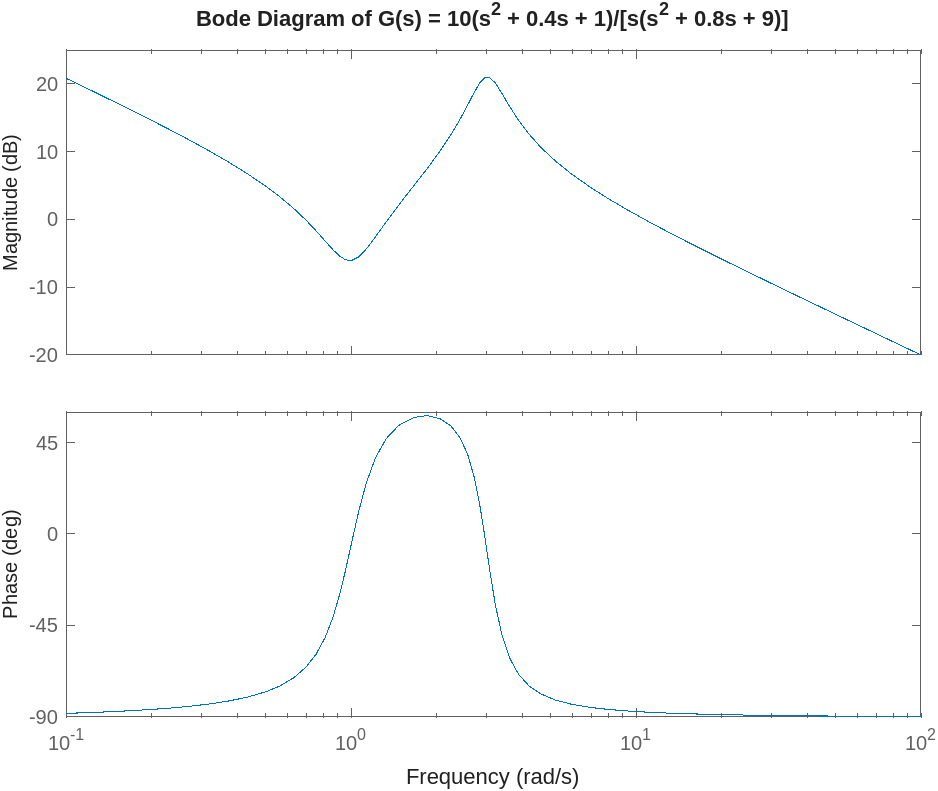
\includegraphics[width=0.85\textwidth]{/Users/arfaz/Desktop/ThirdYearEngineering/2 Fall 2024/1 ECE 360 A01 B05/1 Q-As/MatLab Files/A7/ECE360-B-7-4.png}
%    \caption{Bode Diagram of \( G(s) = \frac{10(s^2 + 0.4s + 1)}{s(s^2 + 0.8s + 9)} \)}
%\end{figure}